\documentclass{book}
\usepackage{import}
\usepackage{preamble}
\usepackage{subfiles}
\title{CluE}

\author{Samuel Meier Jahn}

\begin{document}
%
\begin{figure} [H]
	\centering
	
\includegraphics[width=0.5\linewidth]{figs/fig_CluE_Oxide_logo.png}
  %\caption{}
  \label{fig:clue_logo}
\end{figure}
%
CluE Oxide (Cluster Evolution Oxide) is a open source program for simulating 
electron spin decoherence ab initio using the Cluster Correlation Expansion 
\cite{2008_Yang_Liu,2009_Yang_Liu}.  
CluE Oxide takes as inputs a pbd file and an options file.
The pdb file specifies the coordinates and elements types of all the atoms, 
and the options file specifies all the additional information needed, 
such as the pulse sequence the applied magnetic field, the central spin
coordinates and so on.
%===============================================================================
\section{Overview}
%===============================================================================
The first steps CluE Oxide takes is to read the options and PDB files to construct
the spin system.  This includes applying periodic boundary conditions, and
dropping non-magnetic nuclei as well as those beyond the system radius 
specified in the options.  Isotope substitutions can also be applied at this
step, if specified in the input options.  In addition to isotope substitution,
atoms can be replaced with voids at a chosen rate.  
This can be helpful in hydrogen rich media,
where the proton may be diluted, but including all the deuterons in the
simulation would be too expensive.  The main time cost advantage of dropping 
the deuterons comes in when numerically integrating the Sch{\"o}dinger 
equation, but for large systems a Bernoulli trial at each atom is also
expensive.  Algorithmically, time is saved by avoiding $N$ Bernoulli trials
with a $p$ success rate.  In theses cases CluE Oxide samples a random
number from the binomial distribution parameterized by $N$ and $p$, and then 
selects that many random hydrons to initialize as protons, ignoring the rest.     

Once the system is set up, CluE Oxide construct the tensors for the active spins,
based on the user input.  CluE Oxide will default to applying the point-dipole 
approximation for spin-spin coupling, but the hyperfine tensors can be 
explicitly set to custom values.  
Nuclear electric quadrupole coupling tensors can also be set, but default to 
zero.  Tensor specification requires the eigenvalues, two eigenvectors,
and which atoms to apply the tensor.

CluE Oxide has a grouping algorithm that allows atoms to be specified by a combination 
of properties found in the PDB file, such as element, serial number, or residue,
among others.  The groups can either require or forbid qualifiers.
  
If unspecified CluE Oxide will assume that the applied magnetic field points
along the $z$-direction of the PDB frame, different orientations can be
specified.  Additionally, CluE Oxide can compute the orientation averaged signal.
CluE Oxide can average over custom orientation with custom weights, 
or it use random orientations (inefficient but simple) 
as well as orientations from a Lebedev grid, which integrates exactly 
the orientation dependence of the lowest order terms in a 
polynomial or spherical harmonic expansion\cite{1999_Lebedev}.  
Both the spin Hamiltonian and the Lebedev grid have inversion symmetry; 
this is leveraged to cut the number of calculation in half.

For each orientations, the set of clusters to be included in the $n$-CCE 
simulations must be calculated.  The clusters are the subsets of the system
that contain the central spin (only implicitly included since it is always 
there), and up to $n$ bath spins that form a connected graph, where edges are
defined between two bath spin when they are within some user specified cutoff.
Several cutoff options are available, including 
an orientation independent distance cutoff, 
an orientation dependent dipole-dipole coupling, $\Delta A$, and others
based on the analytic solution of a simplified three spin system.

For large simulations, the primary time cost in CluE Oxide is often from 
diagonalizing and propagating the cluster Hamiltonians.  
In prototyping, a frequency-space method similar to that of \cite{2009_Stoll}
was tried, but likely due to the need to perform both 
a Fourier transform and inverse Fourier transform for each cluster, 
the time-domain integration of the Schr{\"o}dinger equation is more efficient.
The method CluE Oxide employ is to first diagonalize both
electron spin-manifold Hamiltonians separately:
%
\begin{equation}
\hat{H}(\ms) 
= 
\sum_{n } 
\ket{\psi(\ms)}
E_n(\ms)
\bra{\psi(\ms)}
.
\end{equation}
% 
And to construct the propagators in the eigenbasis for a small time increment,
$\delta t$.
%
\begin{equation} \label{eqn07:CluE:propagator}
\hat{U}(\delta t, \ms) 
= 
\sum_{n } 
\ket{\psi(\ms)}
\exp \Big(-\ii \frac{E_n(\ms)  \delta t }{\hbar} \Big)
\bra{\psi(\ms)}
.
\end{equation}
% 
This means that each cluster Hamiltonian only needs to be diagonalized once, 
as the later time propagators can be found via matrix multiplication. 
%
\begin{equation}
\hat{U}(n_t \delta t, \ms) = 
\hat{U}(\delta t, \ms)^{n_t}. 
\end{equation}
%
For some some of the longer time traces, it is helpful to have a small 
$\delta t$ at early times and a longer $\delta t$ at later times.  
The way CluE Oxide addresses this is allow multiple values of $\delta t$ 
accompanied by the number of times each $\delta t$ should be used.  
This requires that multiple propagators be calculated, 
but since the eigenvector have already been
calculated, equation (\ref{eqn07:CluE:propagator}) can be used for multiple
$\delta t$s for a single diagonalization step.

Next at each time point in the simulated experiment, a total  pulse sequence
propagator is calculated as
%
\begin{equation}
\hat{U}_{n_t,\ms} = 
\mathscr{T} \prod_{p} \op{U}(\delta t, {\ms}_p)^{n_t}
,
\end{equation}
%
where by using the $\op{U}(\delta t, {\ms}_p)^{n_t-1}$ from the
previous steps, the cost scaling with the number of timepoints is linear. 
of each $n_t$ is roughly the same. 

The Heisenberg picture detection operator, $\hat{S}_{+}(t)$ in the high 
magnetic field limit, where the Zeeman basis is approximately the electron
spin eigenbasis, can be written solely in terms of the propagators for the
cluster in the as
%
\begin{equation}
\hat{S}_+(n_t) = 
\hat{U}_{n_t,\ms'}^{\dagger} \hat{U}_{n_t,\ms}  
.
\end{equation}
%

For square $d$ by $d$ matrices $A$ and $B$, the inner product between them is
%
\begin{equation}
\braket{A,B} := \tr(A^\dagger B).
\end{equation}
%
To see why this definition makes sense, let $n$ index the elements of the
matrices.  How exactly $n$ indexes the matrices is unimportant as long as it is 
a consistent bijection between the $d^2$ row column pairs and $d^2$ integers.
One possibility is that $n = r + dc$, where $r,c\in [0,d-1]$ 
are the row and column indices respectfully.  In element-wise summation, the
trace is
%
\begin{equation}
\tr(A^\dagger B) = \sum_{r,c} A_{r,c}^{*}B_{c,r}
.
\end{equation}
%
And the inner product between vectors is 
%
\begin{equation}
\braket{A,B} = \sum_{n} A_{n}^{*}B_{n}
.
\end{equation}
%
Since there is a bijection between $n$ and $(r,c)$, 
these expression are equivalent; however, if only the trace is desired and not
the matrix $AB$ itself, the inner product method requires fewer steps, 
and is how CluE Oxide evaluates $\tr\Big(\hat{\rho} \hat{S}_{+}(t)\Big)$.

After all the cluster signals are calculated the CCE auxiliary signals and 
products can be constructed.  By the nature of the product, when calculating 
the $n$-CCE signal, all the $n'$-CCE signals, $n'<n$ are also calculated and 
saved.

If only a single orientation and isotopologue are requested, 
then CluE Oxide ends at this point.  
Different orientations require going back to the orientation
generation step, and different isotopologues require rebuilding the system.
After averaging over all the requested variations, 
CluE Oxide's primary returned data are
the time domain signal $n$-CCE signal and the time axis.  Depending on the 
input options other data may be saved, such as the clusters or 
individual signals from each orientation, the auxiliary signals, 
and system statistics including individual spin and methyl contributions.  
%===============================================================================
\section{Software}
%===============================================================================

%-------------------------------------------------------------------------------
\subsection{Installing}
%-------------------------------------------------------------------------------
To start, please make sure that Rust is installed and up to date\cite{rust}.
Before starting, it is a good idea to run the test suite.
% - - - - - - - - - - - - - - - - - - - - - - - - - - - - - - - - - - - - - - -
\begin{lstlisting}[frame=single,numbers=left,language=bash]
cargo test
\end{lstlisting}
% - - - - - - - - - - - - - - - - - - - - - - - - - - - - - - - - - - - - - - -
A few of the tests rely on random number generations and can occasionally fail.
If this happens try running a second time: they should pass most of the time.
To compile run the following.
% - - - - - - - - - - - - - - - - - - - - - - - - - - - - - - - - - - - - - - -
\begin{lstlisting}[frame=single,numbers=left,language=bash]
cargo build --release
\end{lstlisting}
% - - - - - - - - - - - - - - - - - - - - - - - - - - - - - - - - - - - - - - -
The compiled binary should be in \textit{target/release/} and ready to use.
An optional step is to make sure CluE Oxide is easy to access from 
the command line.
One way to do this on Linux is make an alias by adding the following to 
the .bash\_aliases file.
% - - - - - - - - - - - - - - - - - - - - - - - - - - - - - - - - - - - - - - -
\begin{lstlisting}[frame=single,numbers=left,language=bash]
alias clue_oxide="path/to/clue/target/release/clue_oxide"
\end{lstlisting}
% - - - - - - - - - - - - - - - - - - - - - - - - - - - - - - - - - - - - - - -

%-------------------------------------------------------------------------------
\subsection{Running}
%-------------------------------------------------------------------------------
To see the basic usage for CluE Oxide, run the following.
% - - - - - - - - - - - - - - - - - - - - - - - - - - - - - - - - - - - - - - -
\begin{lstlisting}[frame=single,numbers=left,language=bash]
clue_oxide --help
\end{lstlisting}
% - - - - - - - - - - - - - - - - - - - - - - - - - - - - - - - - - - - - - - -
The output is shown below.
% - - - - - - - - - - - - - - - - - - - - - - - - - - - - - - - - - - - - - - -
\begin{lstlisting}[frame=single,numbers=left,language=bash]
Usage:
    clue_oxide input [-o "options"]

Options:
    -h, --help       Prints help information.
    -H, --hide-title Do not display title information.
    -l, --license    Prints license.
    -O, --option     input additional options.
    -V, --version    Prints version information.
    -W, --warrenty   Prints warrenty information.
\end{lstlisting}
% - - - - - - - - - - - - - - - - - - - - - - - - - - - - - - - - - - - - - - -
To run CluE Oxide from the command line, an input file is needed.
The input file format is .txt file, and is supplied to CluE Oxide as shown below. 
% - - - - - - - - - - - - - - - - - - - - - - - - - - - - - - - - - - - - - - -
\begin{lstlisting}[frame=single,numbers=left,language=bash]
clue_oxide input.txt
\end{lstlisting}
% - - - - - - - - - - - - - - - - - - - - - - - - - - - - - - - - - - - - - - -
%-------------------------------------------------------------------------------
\subsection{Examples}
%-------------------------------------------------------------------------------
Before detailing the syntax of the input file, here is an example input for
reference.
% - - - - - - - - - - - - - - - - - - - - - - - - - - - - - - - - - - - - - - -
\begin{lstlisting}[frame=single,numbers=left,language=c]
/*
Example CluE Oxide Input File
*/
input_structure_file = "MD_300K_25ns-30ns_center_0001.pdb";

detected_spin_position = centroid_over_serials([28,29]);
detected_spin_g_matrix = [2.0097, 2.0064, 2.0025];
detected_spin_g_y = diff(group(tempo_n) , group(tempo_o) );
detected_spin_g_x = diff(group(tempo_c1) , group(tempo_c19) );

radius = 25; // angstroms.

pulse_sequence = hahn;
magnetic_field = 1.2; // T.

number_timepoints = [101];
time_increments = [5e-8];

cluster_method = cce;
max_cluster_size = 4;

neighbor_cutoff_3_spin_hahn_mod_depth = 3.23e-5; 
neighbor_cutoff_3_spin_hahn_taylor_4 = 1e17; // (rad/s)^4.

orientation_grid = lebedev(170);

#[group(tempo_h)]
  residues in [TEM];
  elements in [H];

#[spin_properties(tempo_h, 1H)]
  tunnel_splitting = 80e3; // Hz.

#[group(tempo_n)]
  residues in [TEM];
  elements in [N];

#[group(tempo_o)]
  residues in [TEM];
  elements in [O];

#[group(tempo_c1)]
  serials in [1];

#[group(tempo_c19)]
  serials in [19];
  
#[spin_properties(tempo_n, 14N)]
  hyperfine_coupling = [20,20,100]*1e6;
  hyperfine_x = diff(bonded(tempo_c1),bonded(tempo_c19));
  hyperfine_y = diff(particle,bonded(tempo_o));

  electric_quadrupole_coupling = [-0.28, -1.47, 1.75]*1e6;
  electric_quadrupole_x = diff(bonded(tempo_c1),bonded(tempo_c19));
  electric_quadrupole_y = diff(particle,bonded(tempo_o));

#[config]
write_orientation_signals = "";
write_clusters = "";
\end{lstlisting}
% - - - - - - - - - - - - - - - - - - - - - - - - - - - - - - - - - - - - - - -
The input script is not Turing complete, 
but is sufficient for starting CluE Oxide,
and as will be discussed later, CluE Oxide 
can run from Turing complete languages
like Bash, Python, and Rust.
The syntax is inspired by C, C++, Rust, MATLAB and Python:
all normal lines end in semicolons and double slashes indicate that the rest of 
line is a comment.  Block commenting with ``/*'' and ``*/'' also works. 
Pound signs indicate that the following lines are to be interpreted differently.
Line 5 specifies the input structure as a PDB file.  
Line 7 places the detected electron between the nitrogen and oxygen of TEMPO.
Line 8--10 specifies the electron g-matrix.
Line 12 says to only use a 25 \AA~radius sphere of the PDB, 
applying periodic boundary conditions if need be.
Line 14 specifies the pulse sequence to be simulated.
Line 15 declares the applied magnetic field strength in tesla: 
Line 18 defines the time increments used evaluating propagators; 
for Carr-Purcell sequences with $n_{\uppi}$ $\uppi$-pulses, 
the time increment on the returned time-axis will be $(n_{\uppi}+1)\Delta t$.  
the applied magnetic field is always in along the $z$-axis.
Line 20 determines which cluster approximation to use, 
and line 21 specifies the maximum cluster size to be used.
Lines 23 and 24 specify neighbor cutoffs for determining clusters.
Line 27 selects a 170 point Lebedev grid\cite{1999_Lebedev}.
Lines 29--31 declare a group selecting the TEMPO hydrogens.
%
\begin{figure} [H]
	\centering
	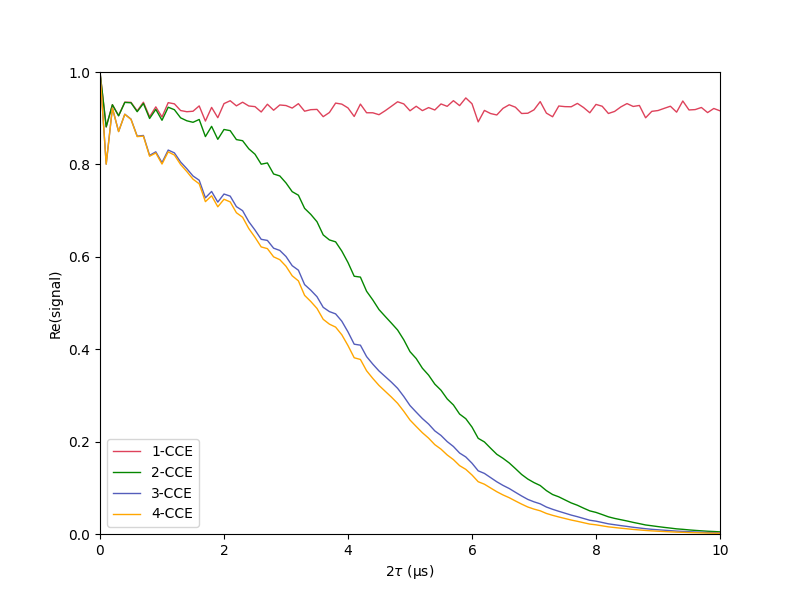
\includegraphics[width=0.75\linewidth]{figs/fig_CluE-sims_n-CCE.png}
  \caption{These Hahn echo simulation show the output of the previous example.
  }
  \label{fig:example_ncce}
\end{figure}
%
%
Each group is required to starts with a 
\textit{\#[group(my\_label)]}, 
followed by various conditions; 
in this case the residue (as indicated in the PDB file),
and the element.
Line 33 and 34 set the methyl tunnel splitting for the TEMPO to 80 kHz,
by referencing the previous group.
This is done by using 
\textit{\#[spin\_properties(my\_label, my\_isotope)]},
where \textit{my\_label} matches the group selecting the TEMPO
hydrogens.
Lines 36--48 declare more groups.
Lines 50--57 sets the TEMPO nitrogen's hyperfine tensor and 
electric quadrupole coupling tensor.
Note that one group is used in 
\textit{\#[spin\_properties(tempo\_n, 14N)]}
to select the TEMPO nitrogen and other groups are used to specify atoms
for orientating the coupling tensors.
Line 59 sets the mode back to \textit{\#[config]}; there is an implied 
\textit{\#[config]} at the start of every CluE Oxide file.
Line 60 and 61 turn off saving orientation dependent signals an clusters,
respectively.
%-------------------------------------------------------------------------------
\section{Input File}
%-------------------------------------------------------------------------------
%-------------------------------------------------------------------------------
\subsection{\#[config]}
%-------------------------------------------------------------------------------
The main section of the input file is \textit{\#[config]}, and is the default
when no mode is declared; however, the line
% - - - - - - - - - - - - - - - - - - - - - - - - - - - - - - - - - - - - - - -
\begin{lstlisting}[frame=single,numbers=left,language=c]
#[config]
\end{lstlisting}
% - - - - - - - - - - - - - - - - - - - - - - - - - - - - - - - - - - - - - - -
will set CluE Oxide to read in \textit{\#[config]} mode and is needed to exit
other modes back to \textit{\#[config]}.
The available fields are explained below.  
% - - - - - - - - - - - - - - - - - - - - - - - - - - - - - - - - - - - - - - -
\begin{center}
\begin{tabular}{| m{20em} | m{1.5cm}| m{7cm} |}
 \hline 
 \textbf{field} & \textbf{values} & \textbf{description} \\ 
  %
 \hline 
 clash\_distance\_pbc & float & 
 minimum distance in \AA~for which particles in periodic boundary condition 
 copies are allowed to overlap particle in the primary cell\\
 %
 \hline 
 cluster\_batch\_size & int & number of clusters to evaluate between saves \\
 %
 \hline 
 cluster\_density\_matrix & den\_mat & 
 method to calculate the density matrix of each cluster\\
 %
 \hline 
 cluster\_method & r2cce, cce & method of evaluating clusters \\
 %
 \hline 
 detected\_g\_matrix & [float; 3] & eigenvalues of the detected spin g-matrix\\
 %
 \hline 
 detected\_g\_x & vector & x-direction of the  detected spin g-matrix\\
 %
 \hline 
 detected\_g\_y & vector & y-direction of the  detected spin g-matrix\\
 %
 \hline 
 detected\_g\_z & vector & z-direction of the  detected spin g-matrix\\
 %
 \hline 
 detected\_spin\_position & spin\_coor 
 & coordinates in \AA~of the detected spin\\
 %
 \hline 
 input\_structure\_file & string & path to the input PDB \\
 %
 \hline 
 load\_geometry & cube, sphere & shape of the spin system \\
 %
 \hline 
 magnetic\_field & float & 
 magnetic field strength in T of the applied magnetic field\\
 %
 \hline 
 max\_cluster\_size & int & maximum cluster size to be evaluated \\
 %
 \hline 
 neighbor\_cutoff\_3\_spin\_hahn\_mod\_depth & float & 
 minimum modulation depth for the three spin hahn echo
 for an edge to be placed between two spins\\
 %
 \hline 
 neighbor\_cutoff\_3\_spin\_hahn\_taylor\_4 & float & 
 minimum magnitude of the $\mathscr{O}\big((2\tau)^4\big)$ coefficient,
 in the three spin hahn echo Taylor series, $|k\omega^4|$,  in (rad/s)$^4$, 
 for an edge to be placed between two spins \\
 %
 \hline 
 neighbor\_cutoff\_coupling & float & 
 minimum $|b_{zz}-2J|$ in Hz 
 for an edge to be placed between two spins\\
 %
 \hline 
 neighbor\_cutoff\_delta\_hyperfine & float & 
 minimum $|\Delta A_{mn}| := |A_{zz,n} - A_{zz,m}|$ in Hz 
 for an edge to be placed between two spins\\
 %
 \hline 
 neighbor\_cutoff\_dipole\_perpendicular & float & 
 minimum $|b_{\perp}|$ in Hz 
 for an edge to be placed between two spins\\
 %
 \hline 
 neighbor\_cutoff\_distance & float & 
 maximum distance in \AA~ 
 for an edge to be placed between two spins\\
 %
 \hline 
 number\_timepoints  & [int] & 
 number of timepoints used for each time increment\\ 
 %
 \hline 
 number\_system\_instances  & int & 
 number of times the system will be simulated\\ 
 %
 \hline 
 orientation\_grid  & ori\_grid & grid used for orientation averaging\\ 
 %
 \hline 
 pulse\_sequence & cp-$n_{\uppi}$, hahn & 
 pulse sequence to simulate with $n_{\uppi}$ $\uppi$-pulses\\
 %
 \hline 
 radius & float & 
 radius in \AA~from the average position of the detected spin to use\\
 %
 \hline 
 save\_dir & string & 
 directory where data will be saved\\
 %
 \hline 
 time\_increments  & [float] & 
 list of $\Delta \tau$s in s used for propagation\\ 
 %
 \hline 
 write\_auxiliary\_signals & string & 
 file name to save cluster auxiliary signals under\\
 %
 \hline 
 write\_bath & string & 
 file name to save bath spins under\\
 %
 \hline 
 write\_clusters & string & 
 file name to save clusters under\\
 %
 \hline 
 write\_info & string & 
 directory name to save general information under\\
 %
 \hline 
 write\_exchange\_groups & string & 
 file name to save exchange groups (such as methyls) under\\
 %
 \hline 
 write\_structure\_pdb & string & 
 PDB file name to save the spin system under\\
 %
 \hline 
\end{tabular}
\end{center} 
\subsubsection{ClusterDensityMatrix} % -----------------------------------------
If no \textit{cluster\_density\_matrix} is specified, the infinite temperature
limit is assumed for the bath spin, so that the density matrix is proportional
to the identity matrix.  To specify a particular temperature, $T$, in kelvin, 
use
% - - - - - - - - - - - - - - - - - - - - - - - - - - - - - - - - - - - - - - -
\begin{lstlisting}[frame=single,numbers=left,language=c]
cluster_density_matrix = thermal(T);
\end{lstlisting}
% - - - - - - - - - - - - - - - - - - - - - - - - - - - - - - - - - - - - - - -

\subsubsection{ClusterMethod} % ---------------------------------------------
There are two cluster evolutions schemes available in CluE Oxide, 
\textit{cce}, and \textit{r2cce}.
The \textit{cce} method implements ensemble CCE
\cite{2008_Yang_Liu,2009_Yang_Liu} and has no explicit limit on the maximum
cluster size.  
The \textit{r2cce} method is a restricted version of CCE, 
using the analytic solution to the simplified three spin model from
\cite{2006_Witzel_DasSarma}, and is therefore limited to a cluster size of two.

% - - - - - - - - - - - - - - - - - - - - - - - - - - - - - - - - - - - - - - -
\begin{lstlisting}[frame=single,numbers=left,language=c]
temperature = 20; // K.
\end{lstlisting}
% - - - - - - - - - - - - - - - - - - - - - - - - - - - - - - - - - - - - - - -
This will switch CluE Oxide from using the identity matrix to the thermal 
density matrix. 

\subsubsection{DetectedSpinCoordinates} % -------------------------------------
The detected spin coordinates have several ways to specified.
They can be specified directly.
% - - - - - - - - - - - - - - - - - - - - - - - - - - - - - - - - - - - - - - -
\begin{lstlisting}[frame=single,numbers=left,language=c]
detected_spin_position = [1.2, -3, 0];
\end{lstlisting}
% - - - - - - - - - - - - - - - - - - - - - - - - - - - - - - - - - - - - - - -
They can be specified as the centroid of atoms in the PDB file.
% - - - - - - - - - - - - - - - - - - - - - - - - - - - - - - - - - - - - - - -
\begin{lstlisting}[frame=single,numbers=left,language=c]
detected_spin_position = centroid_over_serials([28,29]);
\end{lstlisting}
% - - - - - - - - - - - - - - - - - - - - - - - - - - - - - - - - - - - - - - -
Both of these methods assume that the detected spin is localized to a single
point.  If the spin is delocalized of multiple points, a csv file can be used
to provide $|\Psi(x,y,z)|^2$.  
% - - - - - - - - - - - - - - - - - - - - - - - - - - - - - - - - - - - - - - -
\begin{lstlisting}[frame=single,numbers=left,language=c]
detected_spin_position = read_csv("xyzw.csv");
\end{lstlisting}
% - - - - - - - - - - - - - - - - - - - - - - - - - - - - - - - - - - - - - - -
Each row of the file "xyzw.csv" should be four comma separated floating point
numbers, specifying the $x$, $y$, $z$ and weight,
$w = |\Psi(x,y,z)|^2 \d x \d y \d z$, for the coordinates.

\subsubsection{LoadGeometry} % ---------------------------------------------
The \textit{load\_geometry} can be either \textit{sphere}, 
which is the default, or \textit{cube}.  The \textit{sphere} 
\textit{load\_geometry} includes only bath particle that are within the
specified \textit{radius} of the detected spin.  The \textit{cube} 
\textit{load\_geometry} includes all bath particles from all periodic 
boundary duplicates.  
Periodic boundary duplicates are constructed as rectangular prism where there
are $1 + 2\text{ceil}(r/a)$ cell along each dimension, 
where $r$ is the \textit{radius} and $a$ in the cell edge length along the
dimension in question. 

\subsubsection{OrientationGrid} % ---------------------------------------------
The orientation grid specifies the directions and weights for the applied 
static magnetic field.  If no grid is given, the magnetic field is directed 
along the $z$-axis of the PDB file.
A lebedev grid \cite{1999_Lebedev} can be specified.
% - - - - - - - - - - - - - - - - - - - - - - - - - - - - - - - - - - - - - - -
\begin{lstlisting}[frame=single,numbers=left,language=c]
orientation_grid = lebedev(302);
\end{lstlisting}
% - - - - - - - - - - - - - - - - - - - - - - - - - - - - - - - - - - - - - - -
A random grid is also an option.  Here is an example of using a single random
direction. 
% - - - - - - - - - - - - - - - - - - - - - - - - - - - - - - - - - - - - - - -
\begin{lstlisting}[frame=single,numbers=left,language=c]
orientation_grid = random(1);
\end{lstlisting}
% - - - - - - - - - - - - - - - - - - - - - - - - - - - - - - - - - - - - - - -
And as with the detected spin position, a csv file $x$, $y$, $z$ and weight
entries can be used for a custom grid.
% - - - - - - - - - - - - - - - - - - - - - - - - - - - - - - - - - - - - - - -
\begin{lstlisting}[frame=single,numbers=left,language=c]
orientation_grid = read_csv("xyzw.csv");
\end{lstlisting}
% - - - - - - - - - - - - - - - - - - - - - - - - - - - - - - - - - - - - - - -

\subsubsection{PulseSequence} % ---------------------------------------------
To simulate a Carr-Purcell pulse sequence with two $\uppi$-pulses   
% - - - - - - - - - - - - - - - - - - - - - - - - - - - - - - - - - - - - - - -
\begin{lstlisting}[frame=single,numbers=left,language=c]
pulse_sequence = cp-2;
\end{lstlisting}
% - - - - - - - - - - - - - - - - - - - - - - - - - - - - - - - - - - - - - - -
A Hahn echo can be selected as shown. 
% - - - - - - - - - - - - - - - - - - - - - - - - - - - - - - - - - - - - - - -
\begin{lstlisting}[frame=single,numbers=left,language=c]
pulse_sequence = hahn;
\end{lstlisting}
% - - - - - - - - - - - - - - - - - - - - - - - - - - - - - - - - - - - - - - -
Or a Hahn echo is also a Carr-Purcell pulse sequence with one $\uppi$-pulse.
% - - - - - - - - - - - - - - - - - - - - - - - - - - - - - - - - - - - - - - -
\begin{lstlisting}[frame=single,numbers=left,language=c]
pulse_sequence = cp-1;
\end{lstlisting}
% - - - - - - - - - - - - - - - - - - - - - - - - - - - - - - - - - - - - - - -
 
\subsubsection{SystemInstance} % ---------------------------------------------
For simulations with random elements, such as a randomized isotope
distribution, running the over multiple instances can be important.
For example to run the simulation 1000 times each with a random direction,
use the following.  
% - - - - - - - - - - - - - - - - - - - - - - - - - - - - - - - - - - - - - - -
\begin{lstlisting}[frame=single,numbers=left,language=c]
number_system_instances = 1000;
orientation_grid = random(1);
\end{lstlisting}
% - - - - - - - - - - - - - - - - - - - - - - - - - - - - - - - - - - - - - - -
Note that this is different from the following.
% - - - - - - - - - - - - - - - - - - - - - - - - - - - - - - - - - - - - - - -
\begin{lstlisting}[frame=single,numbers=left,language=c]
number_system_instances = 1;
orientation_grid = random(1000);
\end{lstlisting}
% - - - - - - - - - - - - - - - - - - - - - - - - - - - - - - - - - - - - - - -
The former chooses a random isotopologue and a random direction 1000 times,
while the latter uses a single random isotopologue but 10000 random directions.
As an in between, the following chooses 900 random isotopologues, and for
each of them chooses 100 random orientations.
% - - - - - - - - - - - - - - - - - - - - - - - - - - - - - - - - - - - - - - -
\begin{lstlisting}[frame=single,numbers=left,language=c]
number_system_instances = 900;
orientation_grid = random(100);
\end{lstlisting}
% - - - - - - - - - - - - - - - - - - - - - - - - - - - - - - - - - - - - - - -

\subsubsection{TimeAxis} % --------------------------------------------
The time-axis is specified in two part, the number of timepoints, and 
the time increments.  For example, the CluE Oxide input file could include the
following.  
% - - - - - - - - - - - - - - - - - - - - - - - - - - - - - - - - - - - - - - -
\begin{lstlisting}[frame=single,numbers=left,language=c]
number_timepoints = [101,90];
time_increments = [5,50]*1e-9; // seconds.
\end{lstlisting}
% - - - - - - - - - - - - - - - - - - - - - - - - - - - - - - - - - - - - - - -
CluE Oxide will read this and use $\Delta t = 5$ ns for the first 101 timepoints,
and then $\Delta t = 50$ ns for the remaining 90 timepoints.  
There will be 191 timepoints total.  Note that these are the $\Delta t$s for 
the smallest propagator unit, so a Carr-Purcell pulse sequence with $n_\uppi$
$\uppi$-pulses will have a $\Delta t_\text{axis} = (n_\uppi +1 )\Delta t$.
So if the above example is for a Hahn echo ($n_\uppi = 1$), 
$\Delta t_\text{axis} = 10$ ns for the first 101 timepoints $\in [0, 1]\ \upmu$s 
and then $\Delta t_\text{axis} = 100$ ns for the next 90 timepoints
$\in [1.1, 10]\ \upmu$s.

\subsubsection{VectorSpecifiers} % --------------------------------------------
The fields that require values of ``vector'' have several options.
First, a vector can be a list.
% - - - - - - - - - - - - - - - - - - - - - - - - - - - - - - - - - - - - - - -
\begin{lstlisting}[frame=single,numbers=left,language=c]
detected_g_x = [1,0,0];
detected_g_z = [0,0,1];
\end{lstlisting}
% - - - - - - - - - - - - - - - - - - - - - - - - - - - - - - - - - - - - - - -
Note that exactly two axes should be specified: 
the third axis is found with the appropriate cross product.  
The specified axes do not need to be normalized or perfectly orthogonal, 
since CluE Oxide will orthonormalize the vectors itself.  
The reason for this is allow for directions to be specified by properties of
the system.    
The following lines say to use the difference between the atoms in the
\textit{group(tempo\_c1)}, and the atoms in \textit{group(tempo\_c19)} 
for the $x$-direction,
and to use difference between the atoms in the
\textit{group(tempo\_n)}, and the atoms in \textit{group(tempo\_o)} 
for the $y$-direction.
Filters are explained in the next section, but the union of the atoms within
the \textit{diff()} must contain exactly two atoms for a unique vector to
be specified.
% - - - - - - - - - - - - - - - - - - - - - - - - - - - - - - - - - - - - - - -
\begin{lstlisting}[frame=single,numbers=left,language=c]
detected_g_x = diff(group(tempo_c1) , group(tempo_c19) );;
detected_g_y = diff(group(tempo_n) , group(tempo_o) );;
\end{lstlisting}
% - - - - - - - - - - - - - - - - - - - - - - - - - - - - - - - - - - - - - - -
%-------------------------------------------------------------------------------
\subsection{\#[group(my\_label)]}
%-------------------------------------------------------------------------------
The options file can have zero, one, or multiple 
\textit{\#[group(my\_label)]} sections.  
Each \textit{\#[group(my\_label)]} section must have a unique label,
by replacing \textit{my\_label} with the desired label. 
Under the \textit{\#[group(my\_label)]} header, 
the group conditions that can have multiple matches 
are listed as
% - - - - - - - - - - - - - - - - - - - - - - - - - - - - - - - - - - - - - - -
\begin{lstlisting}[frame=single,numbers=left,language=c]
property in [allowed_value_1, allowed_value_n, ...];
\end{lstlisting}
% - - - - - - - - - - - - - - - - - - - - - - - - - - - - - - - - - - - - - - -
or
% - - - - - - - - - - - - - - - - - - - - - - - - - - - - - - - - - - - - - - -
\begin{lstlisting}[frame=single,numbers=left,language=c]
property not in [forbidden_value_1, forbidden_value_n, ...];
\end{lstlisting}
% - - - - - - - - - - - - - - - - - - - - - - - - - - - - - - - - - - - - - - -
The distance group only takes maximum and minimum values and is specified 
as  
% - - - - - - - - - - - - - - - - - - - - - - - - - - - - - - - - - - - - - - -
\begin{lstlisting}[frame=single,numbers=left,language=c]
distance <= r_max; // angstroms
distance >= r_min; // angstroms
\end{lstlisting}
% - - - - - - - - - - - - - - - - - - - - - - - - - - - - - - - - - - - - - - -
where \textit{r\_max} and \textit{r\_min} are floating point numbers
specifing the maximum and minimum distances in \AA~from the detected spin
that the particles in the group can be.
CluE Oxide will find all the spins that fit all specified criteria.
Note that depending upon how the criteria are defined it is possible that
some spins will fall under multiple groups. 
CluE Oxide treats this case as an error and will indicate as such. 
To resolve this error, the group criteria should be refined.
The following table shows the possible group criteria.
% - - - - - - - - - - - - - - - - - - - - - - - - - - - - - - - - - - - - - - -
\begin{center}
\begin{tabular}{| m{20em} | m{1.5cm}| m{7cm} |}
 \hline 
 \textbf{field} & \textbf{values} & \textbf{description} \\ 
 %
 \hline 
 bonded\_elements & [H,He,...] & elements of bonded atoms 
 to match (in) or avoid (not in)\\
 %
 \hline 
 bonded\_residues & [GLY,...] & residues of bonded atoms 
 as specified in the PDB file to match (in) or avoid (not in)\\
 %
 \hline 
 bonded\_serials & [int] & PDB serial numbers of bonded atoms 
 to match (in) or avoid (not in)\\
 %
 \hline 
 bonded\_residue\_sequence\_numbers & [int] & PDB residues sequence numbers 
 of bonded atoms to match (in) or avoid (not in)\\
 %
 \hline 
 distance & float & maximum (<=) or minimum (>=) allowed distance in 
 \AA~from the detected spin
 \\
 %
 \hline 
 elements & [H,He,...] & elements to match (in) or avoid (not in)\\
 %
 \hline 
 extracells & none & restrict to unit cells other than the primary cell\\
 %
 \hline 
 primary\_cell & none & restrict to the primary unit cell\\
 %
 \hline 
 residues & [GLY,...] & residues as specified in the PDB file
 to match (in) or avoid (not in)\\
 %
 \hline 
 residue\_sequence\_numbers & [int] & residues sequence numbers 
 as specified in the PDB file to match (in) or avoid (not in)\\
 %
 \hline 
 serials & [int] & serial numbers as specified in the PDB file
 to match (in) or avoid (not in)\\
 %
 \hline 
\end{tabular}
\end{center}  
%-------------------------------------------------------------------------------
\subsection{\#[structure\_properties(my\_label)]}
%-------------------------------------------------------------------------------
The options file can have zero, one, or multiple 
\textit{\#[structure\_properties(my\_label)]} sections,
where \textit{my\_label} should match to a 
\textit{\#[group(my\_label)]}.
The properties specified under  
\textit{\#[structure\_properties(my\_label)]} will be applied
to all spins that fall under the corresponding
\textit{\#[group(my\_label)]}.
The following table shows the available properties.
% - - - - - - - - - - - - - - - - - - - - - - - - - - - - - - - - - - - - - - -
\begin{center}
\begin{tabular}{| m{20em} | m{1.5cm}| m{7cm} |}
 \hline 
 \textbf{field} & \textbf{values} & \textbf{description} \\ 
 %
 \hline 
 isotope\_abundances & \{1H: 0.9, 2H: 0.1\} & possible isotopes and
 probabilities\\
 %
 \hline 
 void\_probability & float & chance that each particle will be removed\\
 %
 \hline 
\end{tabular}
\end{center} 
% - - - - - - - - - - - - - - - - - - - - - - - - - - - - - - - - - - - - - - -

%-------------------------------------------------------------------------------
\subsection{\#[spin\_properties(my\_label, my\_isotope)]}
%-------------------------------------------------------------------------------
The options file can have zero, one, or multiple 
\textit{\#[spin\_properties(my\_label, my\_isotope)]} 
sections, where \textit{my\_label} should match to a 
\textit{\#[group(my\_label)]}.
The properties specified under  
{\#[spin\_properties(my\_label, my\_isotope)]} will be applied
to all spins of isotope \textit{my\_isotope} that fall under the corresponding
\textit{\#[group(my\_label)]}.
The reason to differentiate between 
\textit{\#[spin\_properties(my\_label, }
\textit{my\_isotope)]}
and \textit{\#[structure\_properties(my\_label)]}
is isotope specificity:
\textit{\#[structure\_properties(my\_label)]} applies to all
particles in the corresponding group, while 
\textit{\#[spin\_properties(my\_label, }
\textit{my\_isotope)]}
only applies to the specified isotope in the corresponding group.
The following table shows the available properties.
% - - - - - - - - - - - - - - - - - - - - - - - - - - - - - - - - - - - - - - -
\begin{center}
\begin{tabular}{| m{20em} | m{1.5cm}| m{7cm} |}
 \hline 
 \textbf{field} & \textbf{values} & \textbf{description} \\ 
 %
 \hline 
 active & bool & 
 specifies if the particle should be used for spin dynamics\\
 %
 \hline 
 electric\_quadrupole\_coupling & [float; 3] & 
 eigenvalues in Hz of the electric quadrupole tensor\\
 %
 \hline 
 electric\_quadrupole\_x & 
 vector & $x$-direction of the electric quadrupole tensor\\
 %
 \hline 
 electric\_quadrupole\_y & 
 vector & $y$-direction of the electric quadrupole tensor\\
 %
 \hline 
 electric\_quadrupole\_z & 
 vector & $z$-direction of the electric quadrupole tensor\\
 %
 \hline 
 g\_matrix & [float; 3] & eigenvalues in of the g-matrix\\
 %
 \hline 
 g\_x & vector & $x$-direction of the g-matrix\\
 %
 \hline 
 g\_y & vector & $y$-direction of the g-matrix\\
 %
 \hline 
 g\_z & vector & $z$-direction of the g-matrix\\
 %
 \hline 
 hyperfine\_coupling & [float; 3] & eigenvalues in Hz of the hyperfine tensor\\
 %
 \hline 
 hyperfine\_x & vector & $x$-direction of the hyperfine tensor\\
 %
 \hline 
 hyperfine\_y & vector & $y$-direction of the hyperfine tensor\\
 %
 \hline 
 hyperfine\_z & vector & $z$-direction of the hyperfine tensor\\
 %
 \hline 
 tunnel\_splitting & float & 
 tunnel splitting in Hz for particle in an exchange group \\
 %
 \hline 
\end{tabular}
\end{center} 
% - - - - - - - - - - - - - - - - - - - - - - - - - - - - - - - - - - - - - - -
\subsubsection{VectorSpecifiers} % --------------------------------------------
Two tensor axes must be specified in addition to the coupling. 
For example, the following sets the nitrogen hyperfine coupling to 
$A_{xx} = A_{yy} = 20$ MHz and $A_{zz} = 100$ MHz.  
It defines the $x$-direction of the tensor as the vector between the two
carbons bonded to the nitrogen: since the nitrogen in TEMPO in bonded to only
two carbon the vector is uniquely defined.  The $y$-direction is defined as
between the particle, the nitrogen in this case, and the oxygen that is bonded 
to the particle.
% - - - - - - - - - - - - - - - - - - - - - - - - - - - - - - - - - - - - - - -
\begin{lstlisting}[frame=single,numbers=left,language=c]
#[spin_properties(tempo_n, 14N)]
hyperfine_coupling = [20,20,100]*1e6; // Hz.
hyperfine_x = diff(bonded(tempo_c),bonded(tempo_c));
hyperfine_y = diff(particle,bonded(tempo_o));;
\end{lstlisting}
% - - - - - - - - - - - - - - - - - - - - - - - - - - - - - - - - - - - - - - -

The arguments \textit{diff()} can take are tabulated below.
The table assumes that the user defined 
\textit{\#[group(my\_group)]}.
% - - - - - - - - - - - - - - - - - - - - - - - - - - - - - - - - - - - - - - -
\begin{center}
\begin{tabular}{| m{20em} |  m{7cm} |}
 \hline 
 \textbf{argument} & \textbf{description} \\ 
 %
 \hline 
 bonded(my\_group) & 
 particles that are are in my\_group and bonded to reference particle\\ 
 %
 \hline 
 group(my\_group) & 
 particles that are are in my\_group\\ 
 %
 \hline 
 particle & 
 the reference particle itself\\ 
 %
 \hline 
 same\_molecule(my\_group) & 
 particles that are are in my\_group and in the same molecule as 
 the reference particle\\ 
 %
 \hline 
\end{tabular}
\end{center} 
% - - - - - - - - - - - - - - - - - - - - - - - - - - - - - - - - - - - - - - -
%===============================================================================
\section{Shell Scripting}
%===============================================================================
The previous interface is useful for an isolated simulation, 
but to run multiple simulations that are nearly the same except for a few
parameters being investigated, running CluE Oxide as a scrip is helpful.  
To this end there are several methods available.
The first is via a shell script: CluE Oxide allows additional option to be appended
to a base options file with the ``-O'' flag.  
Here is an example  Bash script to run several different input structures
with the same setting.
% - - - - - - - - - - - - - - - - - - - - - - - - - - - - - - - - - - - - - - -
\begin{lstlisting}[frame=single,numbers=left,language=bash]
#!/usr/bin/bash

clue="path/to/clue"

options="path/to/options.txt"

files=( 
    structure_1.pdb
    structure_2.pdb
    structure_n.pdb
)
for file in "${files[@]}"; do
    $clue $options -O "\"input_structure_file = $file;\""
done
\end{lstlisting}
% - - - - - - - - - - - - - - - - - - - - - - - - - - - - - - - - - - - - - - -
Note that CluE Oxide interprets this the same as just appending 
the options to the end of the options file,
the command line options must be be compatible with the options file.
This means that the option should not already be set in the options file,
and that the options file leaves off in the correct mode.
For example if ``\#[config]'' options are to be set, the options file should
not end in another mode like ``\#[group(label=my\_label)]''.

%===============================================================================
\section{pyCluE}
%===============================================================================
Additionally, CluE Oxide has a Python interface.
%-------------------------------------------------------------------------------
\subsection{Installing}
%-------------------------------------------------------------------------------
Within the CluE Oxide source directory, navigate to the pyclue directory.
% - - - - - - - - - - - - - - - - - - - - - - - - - - - - - - - - - - - - - - -
\begin{lstlisting}[frame=single,numbers=left,language=bash]
cd pyclue
\end{lstlisting}
% - - - - - - - - - - - - - - - - - - - - - - - - - - - - - - - - - - - - - - -
The Python interface uses maturin\cite{maturin} to compile.
% - - - - - - - - - - - - - - - - - - - - - - - - - - - - - - - - - - - - - - -
\begin{lstlisting}[frame=single,numbers=left,language=bash]
cd pyclue
python3 -m venv <path/to/virtual/environment>
source <path/to/virtual/environment/bin/activate>
pip install maturin
maturin build
\end{lstlisting}
% - - - - - - - - - - - - - - - - - - - - - - - - - - - - - - - - - - - - - - -
One potential issue is that when maturin tries to compile CluE Oxide, 
it can fail to see the operating system unique flags, and will try to use them
all.  To account for this, open CluE Oxide's Cargo.toml file and comment out 
everything under the unneeded operating system section.  
For example, to compile on Linux add comments as shown below.
% - - - - - - - - - - - - - - - - - - - - - - - - - - - - - - - - - - - - - - -
\begin{lstlisting}[frame=single,numbers=left,language=bash]
[target.'cfg(unix)'.dependencies]
ndarray-linalg = { version = "0.15", features = ["openblas-static"] }

#[target.'cfg(windows)'.dependencies.ndarray-linalg]
#version = '0.15.0'
#features = ['intel-mkl']
\end{lstlisting}
% - - - - - - - - - - - - - - - - - - - - - - - - - - - - - - - - - - - - - - -
Once built, navigate to \textit{target/wheels}, source the desired
Python environment, and use pip to install the wheel.
% - - - - - - - - - - - - - - - - - - - - - - - - - - - - - - - - - - - - - - -
\begin{lstlisting}[frame=single,numbers=left,language=bash]
cd target/wheels
source <path/to/installation/environment/bin/activate>
pip install <pyclue.whl>
\end{lstlisting}
% - - - - - - - - - - - - - - - - - - - - - - - - - - - - - - - - - - - - - - -
%-------------------------------------------------------------------------------
\subsection{Running}
%-------------------------------------------------------------------------------
Running CluE Oxide via Python is done through the \textit{CluEOptions} class.
% - - - - - - - - - - - - - - - - - - - - - - - - - - - - - - - - - - - - - - -
\begin{lstlisting}[frame=single,numbers=left,language=python]
class clue_oxide.CluEOptions(config = {},group_list =[], structure_properties_list = [], spin_properties_list = [])
\end{lstlisting}
% - - - - - - - - - - - - - - - - - - - - - - - - - - - - - - - - - - - - - - -

% - - - - - - - - - - - - - - - - - - - - - - - - - - - - - - - - - - - - - - -
\begin{center}
\begin{tabular}{| m{12em} | m{3.5cm}| m{7cm} |}
 \hline 
 \textbf{parameter} & \textbf{values} & \textbf{description} \\ 
 %
 \hline
 config & dictionary of strings & general config input\\
 %
 \hline
 group\_list & [Group] & group input\\ 
 %
 \hline
 structure\_properties\_list & [StructureProperties] & 
 non-isotope specific properties input\\ 
 %
 \hline
 spin\_properties\_list & [SpinProperties] & 
 isotope specific properties input\\ 
 %
 \hline 
\end{tabular}
\end{center}
% - - - - - - - - - - - - - - - - - - - - - - - - - - - - - - - - - - - - - - -
The \textit{Group} class signature is shown below.
% - - - - - - - - - - - - - - - - - - - - - - - - - - - - - - - - - - - - - - -
\begin{lstlisting}[frame=single,numbers=left,language=python]
class clue_oxide.Group(label, criteria = {})
\end{lstlisting}
% - - - - - - - - - - - - - - - - - - - - - - - - - - - - - - - - - - - - - - -
The \textit{label} parameter should be a string and serves the same purpose as 
the label in \textit{\#[group(my\_label)]} discussed earlier.
The \textit{criteria} parameter is a dictionary of strings.
Similarly \textit{StructureProperties} in analogous to a 
\textit{\#[structure\_properties(my\_label)]} section.
% - - - - - - - - - - - - - - - - - - - - - - - - - - - - - - - - - - - - - - -
\begin{lstlisting}[frame=single,numbers=left,language=python]
class clue_oxide.StructureProperties(label, properties = {})
\end{lstlisting}
% - - - - - - - - - - - - - - - - - - - - - - - - - - - - - - - - - - - - - - -
And \textit{SpinProperties} in analogous to a 
\textit{\#[spin\_properties(my\_label, my\_isotope)]} section.
% - - - - - - - - - - - - - - - - - - - - - - - - - - - - - - - - - - - - - - -
\begin{lstlisting}[frame=single,numbers=left,language=python]
class clue_oxide.SpinProperties(label, isotope, properties = {})
\end{lstlisting}
% - - - - - - - - - - - - - - - - - - - - - - - - - - - - - - - - - - - - - - -
Note that the additional string, \textit{isotope}, is required.

Below in an example where an MD frame of TEMPO solvated in water is run with
different tunnel splittings.  
Note that the pyCluE specific syntax is similar is similar to the standard 
CluE Oxide input files. 
% - - - - - - - - - - - - - - - - - - - - - - - - - - - - - - - - - - - - - - -
\begin{lstlisting}[frame=single,numbers=left,language=python]
import clue_oxide as clue
import matplotlib
from matplotlib import pyplot as plt
import numpy as np

def main():

  # Initialize options.
  options = clue.CluEOptions(
      config = {
        "input_structure_file": "\"MD_300K_25ns-30ns_center_0001.pdb\"",
        "radius": "25", # angstroms
        "detected_spin_position": "centroid_over_serials([28,29])",
        "detected_spin_g_matrix": "[2.0097, 2.0064, 2.0025]",
        "detected_spin_g_y": "diff(group(tempo_n) , group(tempo_o) )",
        "detected_spin_g_x": "diff(group(tempo_c1) , group(tempo_c19) )",
        "number_timepoints": "[101]",
        "time_increments": "[5e-8]", # s
        "cluster_method": "cce",
        "max_cluster_size": "3",
        "magnetic_field": "1.2", # T
        "pulse_sequence": "hahn",
        "neighbor_cutoff_3_spin_hahn_mod_depth": "3.23e-5",
        "neighbor_cutoff_3_spin_hahn_taylor_4": "1e17", # (rad/s)^4
      },
      group_list = [
        clue.Group("tempo_h", criteria = {
          "residues in": "[TEM]",
          "elements in": "[H]",
        }),
        clue.Group("tempo_n", criteria = {
          "residues in": "[TEM]",
          "elements in": "[N]",
        }),
        clue.Group("tempo_o", criteria = {
          "residues in": "[TEM]",
          "elements in": "[O]",
        }),
        clue.Group("tempo_c1", criteria = {
          "residues in": "[TEM]",
          "elements in": "[C]",
          "serials in": "[1]"
        }),
        clue.Group("tempo_c19", criteria = {
          "residues in": "[TEM]",
          "elements in": "[C]",
          "serials in": "[19]"
        }),
      ],
      spin_properties_list = [
        clue.SpinProperties("tempo_n", "14N", properties = {
          "hyperfine_coupling": "[20,20,100]*1e6", # Hz
          "hyperfine_x": "diff(bonded(tempo_c1),bonded(tempo_c19))",
          "hyperfine_y": "diff(particle,bonded(tempo_o))",
          "electric_quadrupole_coupling": "[-0.28, -1.47, 1.75]*1e6", # Hz
          "electric_quadrupole_x": "diff(bonded(tempo_c1),bonded(tempo_c19))",
          "electric_quadrupole_y": "diff(particle,bonded(tempo_o))",
        }),
      ])


  # Initialize figure.
  plt.rc('font', size=12)
  plt.rc('axes', labelsize=12)

  fig, (ax) = plt.subplots(1,1,figsize=(8, 6) );
  cmap = matplotlib.colormaps['viridis']

  # Set desired methyl tunnel splittings. 
  tunnel_splittings = np.array([0,20,40,80,100])*1e3;

  # Loop over tunnel splittings.
  for nut in tunnel_splittings:

    # Set tunnel splitting.
    options.set_spin_properties("tempo_h", "1H",
        key = "tunnel_splitting", value = f"{nut}")

    # Print CluE input file.
    options.print()
   
    # Run CluE.
    time , signal = options.run()

    # Plot output.
    ax.plot(np.array(time)*1e6,np.real(np.array(signal)),
      color = cmap(nut/max(tunnel_splittings)), linewidth=1);


  # Polish the plot.
  norm = matplotlib.colors.Normalize(vmin=0, vmax=max(tunnel_splittings)*1e-3)
  
  sm = plt.cm.ScalarMappable(cmap=cmap, norm=norm)
  sm.set_array([])

  plt.colorbar(sm, label=r"$\nu_\mathrm{t}$ (kHz)", orientation="vertical")  
  ax.set_xlabel(r"$2\tau$ (μs)");
  ax.set_ylabel("normalized echo amplitude");
  ax.axis([0,10,0,1.0] )

  # Save figure.
  plt.savefig('CluE-sims.png')

if __name__ == "__main__":
  main();
\end{lstlisting}
% - - - - - - - - - - - - - - - - - - - - - - - - - - - - - - - - - - - - - - -
%
\begin{figure} [H]
	\centering
	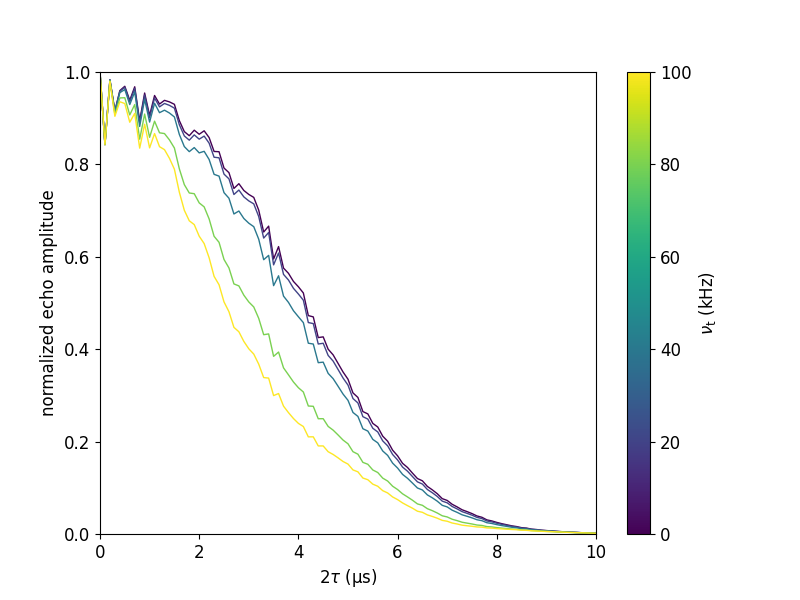
\includegraphics[width=0.75\linewidth]{figs/fig_pyCluE-sims.png}
  \caption{These Hahn echo simulation show the output of the previous example.
  The color-axis indicates the tunnel splitting.
  }
  \label{fig:pyclue_out}
\end{figure}
%
Here the input is modified before sending it to CluE Oxide, 
so settings can be overwritten in the script.
Figure \ref{fig:pyclue_out} shows the output.  
Note that to save on computation time, these simulation are only at the 3-CCE 
level, and only use one frame at a single orientation.
%===============================================================================
\section{Rust}
%===============================================================================
Finally, since CluE Oxide is written in Rust, it is fairly straight forward to 
integrate CluE Oxide into a Rust program. 
Here is a script to run CluE Oxide over different proton concentrations.
The output is shown in figure \ref{fig:rust_out}.
% - - - - - - - - - - - - - - - - - - - - - - - - - - - - - - - - - - - - - - -
\begin{lstlisting}[frame=single,numbers=left,language=c]
use clue_oxide as clue;
use clue_oxide::{
  physical_constants::Isotope,
  config::particle_config::{IsotopeAbundance,IsotopeDistribution}
};

fn main() {

    // Initialize options.
    let config = match clue::config::Config::from("
        input_structure_file = \"TEMPO_wat_gly_70A.pdb\";
        radius = 25; // angstroms.

        detected_spin_position = centroid_over_serials([28,29]);
        detected_spin_g_matrix = [2.0097, 2.0064, 2.0025];
        detected_spin_g_y = diff(group(tempo_n) , group(tempo_o) );
        detected_spin_g_x = diff(group(tempo_c1) , group(tempo_c19) );
        number_timepoints = [101,140];

        time_increments = [50,500]*1e-9;
        cluster_method = cce;
        max_cluster_size = 2;
        magnetic_field = 1.2; // T.
        pulse_sequence = hahn;

        number_system_instances = 10;
        orientation_grid = random(1);

        neighbor_cutoff_distance = 4; // angstroms.

      #[group(tempo_n)]
        residues in [TEM];
        elements in [N];

      #[group(tempo_o)]
        residues in [TEM];
        elements in [O];

      #[group(tempo_c1)]
        serials in [1];

      #[group(tempo_c19)]
        serials in [19];

      #[spin_properties(tempo_n, 14N)]
        hyperfine_coupling = [20,20,100]*1e6;
        hyperfine_x = diff(bonded(tempo_c1),bonded(tempo_c19));
        hyperfine_y = diff(particle,bonded(tempo_o));

        electric_quadrupole_coupling = [-0.28, -1.47, 1.75]*1e6;
        electric_quadrupole_x = diff(bonded(tempo_c1),bonded(tempo_c19));
        electric_quadrupole_y = diff(particle,bonded(tempo_o));

      #[group(solvent_h)]
        residues not in [TEM];
        elements in [H];

      #[structure_properties(solvent_h)]
        isotope_abundances = {1H: 1, 2H: 0};

    "){
      Ok(cfg) => cfg,
      Err(err) => {
        eprintln!("CluE Error: {}.",err);
        return;
      },
    };

 
    // Find where the solvent properties are stored.
    let mut solvent_h_idx: Option<usize> = None;

    for (idx, p_cfg) in config.particles.iter().enumerate(){
      if p_cfg.label == "solvent_h"{
        solvent_h_idx = Some(idx);
        break;
      }
    }

    let solvent_h_idx = solvent_h_idx.expect("Could not find solvent_h_idx.");


    // Initialize desired mole fractions.
    let proton_fractions = vec![1.0, 0.75, 0.5, 0.25, 0.0];

    // Loop over mole fractions.
    for &frac in proton_fractions.iter(){
      
      let mut frac_config = config.clone();

      frac_config.save_name = Some(format!("CluE-proton_frac_{}",frac));

      let properties = frac_config.particles[solvent_h_idx]
        .properties.as_mut().expect("No properties for solvent_h");

      // Set isotope mole fractions.
      let isotope_abundances = vec![
        IsotopeAbundance{isotope: Isotope::Hydrogen1, abundance: frac},
        IsotopeAbundance{isotope: Isotope::Hydrogen2, abundance: 1.0 - frac},
      ];

      properties.isotopic_distribution = IsotopeDistribution{
          isotope_abundances,
          void_probability: None
      };

      // Run CluE.
      match clue::run(frac_config){
        Ok(_) => (),
        Err(err) => eprintln!("CluE Error: {}.",err),
      }
    }
}
\end{lstlisting}
% - - - - - - - - - - - - - - - - - - - - - - - - - - - - - - - - - - - - - - -
%
\begin{figure} [H]
	\centering
	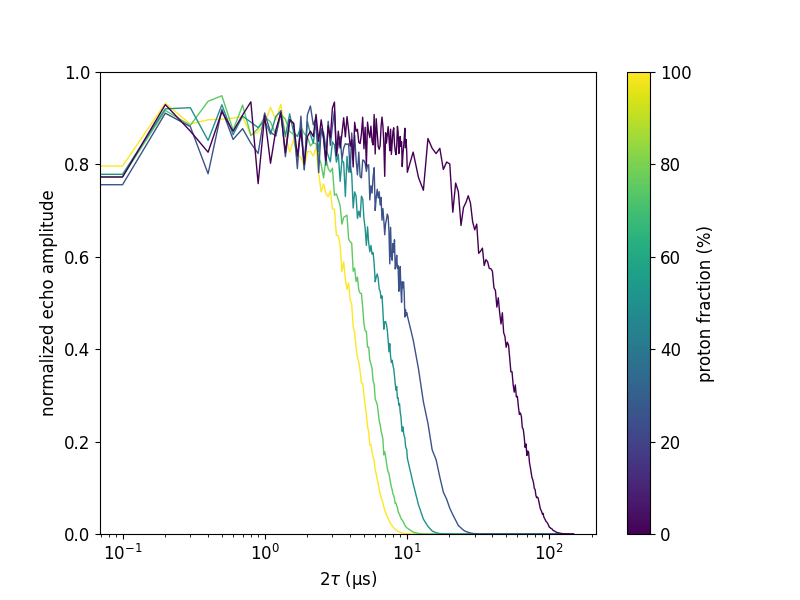
\includegraphics[width=0.75\linewidth]{figs/fig_CluE-proton_fractions.png}
  \caption{These Hahn echo simulation show the output of the previous example.
  The color-axis indicates the proton fraction.
  Note that the $2\tau$-axis is logarithmic.
  }
  \label{fig:rust_out}
\end{figure}
%
The primary way to use CluE Oxide with Rust is to create an instance of 
\textit{Config} and feed it to the run function.
The easiest way to initialize an instance of \textit{Config} is to use 
\textit{Config::from(input: \&str)}; this uses the same syntax as the 
CluE Oxide input files. 
Note that because the each new \textit{frac\_config} is modified after it
has been constructed, the safety check to ensure values are not set multiple 
times is passed and properties can be modified directly.
Every field of \textit{Config} has a data type that is either an 
\textit{Option<T>} or a \textit{Vec::<T>}, for generic type \textit{T}; 
values of \textit{None} or an empty vector are considered unset.
Which entries are required depends on the details of the simulation.
CluE Oxide will return an error explaining what is missing if it needs an option that
is unset.  Several fields have default values, which can be set with the
set\_defaults method.  
Note that set\_defaults will not overwrite user set values.  
This method is called automatically when using the command line or python
interface.
The \textit{Config} struct is defined as shown below, with the defaults shown 
as comments.    
% - - - - - - - - - - - - - - - - - - - - - - - - - - - - - - - - - - - - - - -
\begin{lstlisting}[
frame=single,
numbers=left,
language=c
]
#[derive(Debug,Clone,Default)]
pub struct Config{
  pub clash_distance: Option<f64>,
  pub clash_distance_pbc: Option<f64>,
  pub cluster_batch_size: Option<usize>,
  pub cluster_method: Option<ClusterMethod>,
  pub density_matrix: Option<DensityMatrixMethod>,
  pub detected_spin_g_matrix: Option<TensorSpecifier>,
  pub detected_spin_identity: Option<Isotope>,
  pub detected_spin_multiplicity: Option<usize>,
  pub detected_spin_position: Option<DetectedSpinCoordinates>,
  pub detected_spin_transition: Option<[usize;2]>,
  pub extracell_particles: Vec::<ParticleConfig>,
  pub input_structure_file: Option<String>,
  pub load_geometry: Option<LoadGeometry>,
  pub magnetic_field: Option<Vector3D>,
  pub max_cluster_size: Option<usize>,
  pub neighbor_cutoff_coupling: Option<f64>,
  pub neighbor_cutoff_delta_hyperfine: Option<f64>,
  pub neighbor_cutoff_dipole_perpendicular: Option<f64>,
  pub neighbor_cutoff_distance: Option<f64>,
  pub neighbor_cutoff_3_spin_hahn_mod_depth: Option<f64>,
  pub neighbor_cutoff_3_spin_hahn_taylor_4: Option<f64>,
  pub number_system_instances: Option<usize>,
  pub number_timepoints: Vec::<usize>,
  pub orientation_grid: Option<OrientationAveraging>,
  pub particles: Vec::<ParticleConfig>,
  pub pdb_model_index: Option<usize>,
  pub pulse_sequence: Option<PulseSequence>,
  pub remove_partial_methyls: Option<bool>,
  pub root_dir: Option<String>,
  pub radius: Option<f64>,
  pub rng_seed: Option<u64>,
  pub save_name: Option<String>,
  time_axis: Vec::<f64>,
  pub time_increments: Vec::<f64>,
  pub write_auxiliary_signals: Option<String>, 
  pub write_bath: Option<String>,
  pub write_clusters: Option<String>,
  pub write_info: Option<String>,
  pub write_exchange_groups: Option<String>,
  pub write_orientation_signals: Option<String>,
  pub write_structure_pdb: Option<String>,
  pub write_tensors: Option<String>,
}
\end{lstlisting}
% - - - - - - - - - - - - - - - - - - - - - - - - - - - - - - - - - - - - - - -
\printbibliography
\end{document}
